\documentclass[notheorems,xetex]{beamer}
%\documentclass[UTF8]{ctexbeamer}
\usepackage{xeCJK}%preamble part
%\usepackage{showframe}
\usepackage{amsmath, amsthm, amssymb}
\usepackage{graphicx}
\usepackage{bm}
\usepackage{caption}
\usepackage{ragged2e}
\usepackage{multirow}
\usepackage{float}
\usepackage{color}
\usepackage{listings}
\lstdefinestyle{lstStyleBase}{%
   basicstyle=\small\ttfamily,
   aboveskip=\medskipamount,
   belowskip=\medskipamount,
   lineskip=0pt,
   boxpos=c,
   showlines=false,
   extendedchars=true,
   upquote=true,
   tabsize=2,
   showtabs=false,
   showspaces=false,
   showstringspaces=false,
   numbers=none,
   linewidth=\linewidth,
   xleftmargin=4pt,
   xrightmargin=0pt,
   resetmargins=false,
   breaklines=true,
   breakatwhitespace=false,
   breakindent=0pt,
   breakautoindent=true,
   columns=flexible,
   keepspaces=true,
   gobble=2,
   framesep=3pt,
   rulesep=1pt,
   framerule=1pt,
   backgroundcolor=\color{gray!5},
   stringstyle=\color{green!40!black!100},
   keywordstyle=\bfseries\color{blue!50!black},
   commentstyle=\slshape\color{black!60}}

\lstdefinestyle{lstStyleShell}{%
   style=lstStyleBase,
   frame=l,
   rulecolor=\color{purple},
   language=bash}
%\usepackage[font=Helv,timeinterval=3]{tdclock}
\DeclareMathOperator*{\rgmax}{argmax}
\DeclareMathOperator*{\rgmin}{argmin}
\DeclareMathOperator{\tr}{tr}
%\setCJKmainfont{SimSun}[AutoFakeBold=false]
%\setsansfont{SimSun}
\setbeamertemplate{frametitle}[default][center]
\setbeamertemplate{footline}[frame number]
\setlength{\parindent}{0.8cm}
%\newcommand{\transpose}[1]{\ensuremath{#1^{\scriptscriptstyle T}}}
\usetheme{Lab2C}
\title{一款辅助外语学习的词典} % (optional, use only with long paper titles)
\author[赵丰]
{\quad {赵丰}\\ \and {zhaofeng-shu33}}
\institute[清华大学] % (optional, but mostly needed)
{\normalsize\quad
  2020中文学生开源年会
}
\date{\the\year 年 \the\month 月 \the\day 日}
%\AtBeginSubsection[]
%{
%  \begin{frame}<beamer>{目录}
%    \tableofcontents[currentsection,currentsubsection]
%  \end{frame}
%}


\begin{document}
\frame{\titlepage}
\frame{\tableofcontents}
%\date{\hspace{1mm} \timemark}
\section{背景}
\begin{frame}{项目技术变迁}
\begin{itemize}
	\item 2015 年创立,起初采用 windows 系统的 Qt4 框架
	\item 2016 年提供 web 静态前端,用 jquery 开发
	\item 2017 年用 Django 开发后端服务,在 GitHub 创建 Leidenschaft 组织托管代码
	\item 2020 年,删除部分不兼容的功能,在 \url{http://leidenschaft.cn/django/static/index.html} 上发布德语词典版本
\end{itemize}
\end{frame}
\begin{frame}{关于电子词典}
\begin{description}
	\item[wiktionary] 在线使用,用户贡献词条
	\item[freedict]	词典数据在 Linux 发行版上可直接安装
	\item[mdict] 用户贡献词典
\end{description}
\begin{block}{技术路线}
\begin{itemize}
	\item 数据存储: SQL 数据库 或 词典数据格式
	\item 用户界面: 桌面软件 或 web app
	\item 查询 API: 连接数据存储与用户界面
\end{itemize}
\end{block}
\end{frame}
\section{功能}
\frame{\tableofcontents[currentsection]}
\begin{frame}{查词}

\begin{itemize}
	\item 搜索框
     \begin{figure}
	  \centering
	  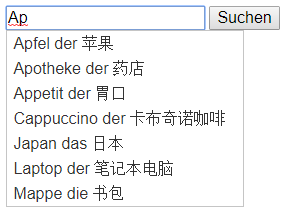
\includegraphics[height=3cm]{search1.png}
	\end{figure}	
	\item 导航栏与词条界面
     \begin{figure}
	\centering
	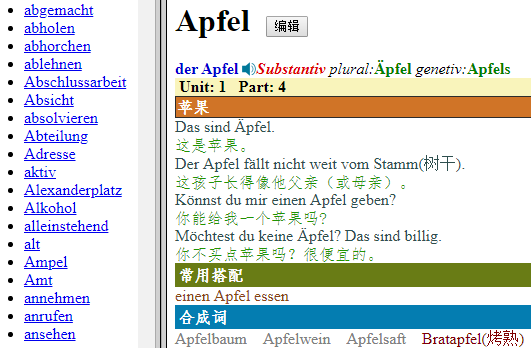
\includegraphics[height=3cm]{search2.png}
	\end{figure}
\end{itemize}
\begin{figure}
	%\includegraphics[height=3.5cm]{example_reset.png}
\end{figure}
\end{frame}

\begin{frame}{添加或修改现有词条}
\begin{figure}
	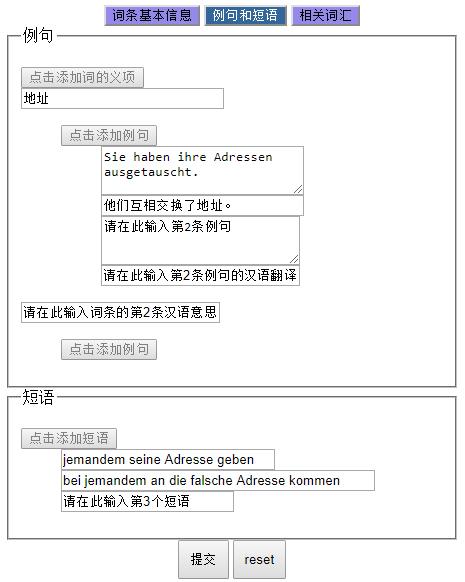
\includegraphics[height=6cm]{edit.png}
	%\caption{numpy 仓库中的 tags}
\end{figure}
\end{frame}
\section{技术栈}
\frame{\tableofcontents[currentsection]}
\begin{frame}{词典数据格式}
\begin{itemize}
\item 采用 XML 的方式存储词条;
\item 用 DTD 规定 XML 的结构;
\item 用 XSLT 渲染 词条至浏览器;
\end{itemize}
\begin{figure}
	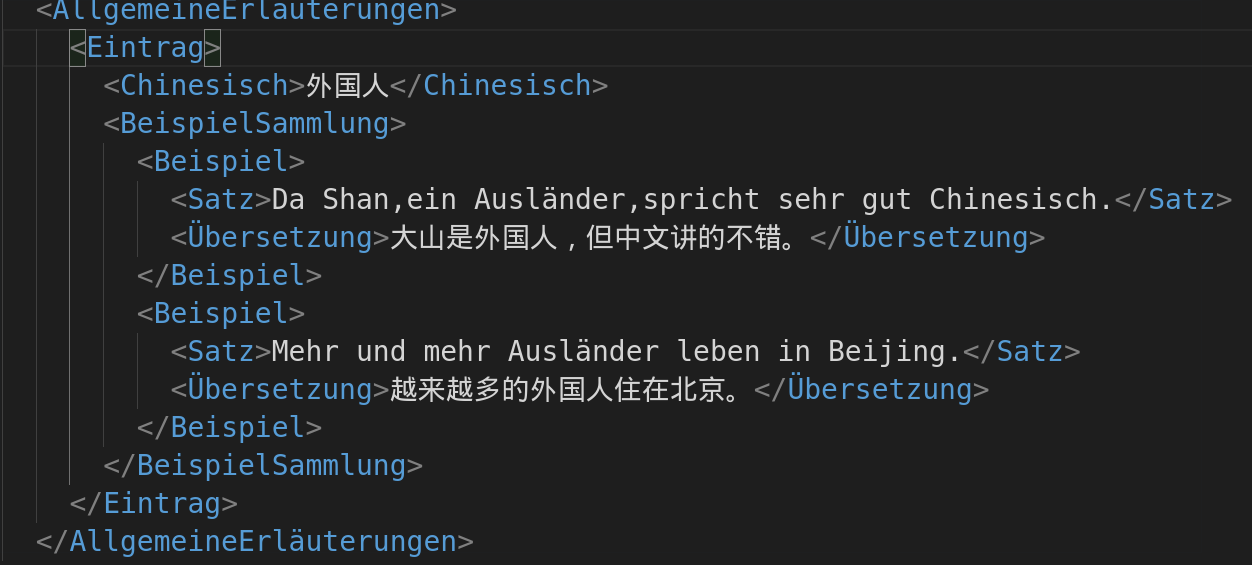
\includegraphics[height=4cm]{xml.png}
	\caption{Ausländer 词条释义项的存储}
\end{figure}

\end{frame}
\begin{frame}[fragile]{DTD 介绍}
\begin{itemize}
	\item 全称是 Document Type Definition
	\item W3C 标准
	\item 规定 XML 的格式
\end{itemize}
\begin{block}{德语中动词完成时态模板}
\begin{lstlisting}[language=bash]
<!ELEMENT Perfekt (ich,du,er_sie_es,wir,ihr,sie_Sie)>
<!ELEMENT ich (#PCDATA)>
<!ATTLIST Perfekt hilfsverb CDATA #REQUIRED>
\end{lstlisting}
\end{block}
\end{frame}
\begin{frame}{XSLT 介绍}
\begin{itemize}
	\item 全称是 eXtensible Stylesheet Language Transformations
	\item W3C 标准
	\item 规定 XML 数据应该怎样渲染成 HTML
\end{itemize}
\begin{figure}
	\centering
	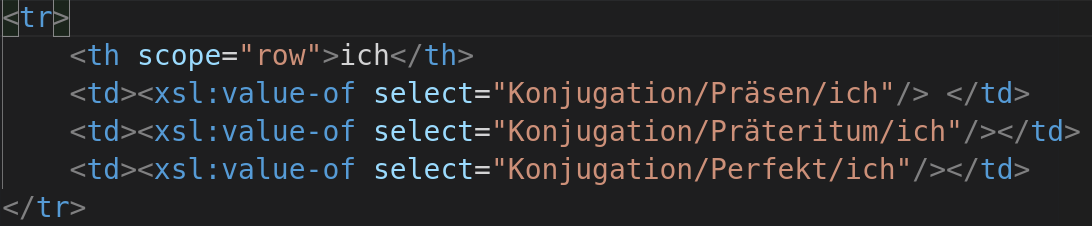
\includegraphics[height=2.5cm]{conjugation.png}
	\caption{渲染动词变位表}
\end{figure}
\end{frame}
\begin{frame}{词典前端界面}
\begin{itemize}
	\item 用 HTML4 进行布局
	\item 用 jquery 进行交互事件处理
	\item 用 ajax 处理创建与编辑请求
\end{itemize}
\begin{figure}
	%\includegraphics[height=2.5cm]{accept_incoming.png}
\end{figure}

\end{frame}
\begin{frame}{其他语言支持}
\begin{itemize}
	\item 最初开发将一些德语特有的词法现象写到了代码里
	\item 正在开发的 2.0 版本将对其他语言提供支持
\end{itemize}
\begin{itemize}
	\item 每种语言有自己的 DTD 模板,比如日语单词的模板中需要有平假名注音的属性
	\item 后端处理创建和更新请求时
\end{itemize}
\begin{figure}
%\includegraphics[height=2.5cm]{recover_changes.png}
\caption{复现效果}
\end{figure}
\begin{center}
feature 分支仅贡献一处改动
\end{center}
\begin{figure}
	%\includegraphics[height=2.5cm]{original.png}
	\caption{原有效果}
\end{figure}
\end{frame}



%\begin{frame}{GitHub Action}

%\end{frame}


\end{document}